\documentclass[a0,landscape]{a0poster}
% --- Постер по проекту. Чистый безрамочный 4-колоночный стиль
% (красные заголовки, белый фон) в духе шаблона MIPT optimization class.

\usepackage[utf8]{inputenc}
\usepackage[T2A]{fontenc}
\usepackage[russian]{babel}
\usepackage{amsmath,amssymb}
\usepackage{multicol}
\usepackage{graphicx}
\usepackage{booktabs}
\usepackage{xcolor}
\usepackage{array}

\definecolor{titlered}{RGB}{176,23,31}
\setlength{\columnsep}{3.5cm}
\setlength{\parindent}{0pt}
\setlength{\parskip}{0.5\baselineskip}

% красный заголовок секции, как в шаблоне
\newcommand{\heading}[1]{\medskip{\color{titlered}\Large\bfseries #1}\par
  \vspace{-0.3\baselineskip}{\color{titlered}\hrule height 1pt}\medskip}

\newcommand{\R}{\mathbb{R}}
\newcommand{\E}{\mathbb{E}}
\newcommand{\norm}[1]{\lVert#1\rVert}
\newcommand{\Sstable}{\mathcal{S}_\alpha}
\DeclareMathOperator{\med}{med}
\DeclareMathOperator{\Var}{Var}

\begin{document}

% ===================== ШАПКА =====================
{\color{titlered}\veryHuge\bfseries
Шумоподавление наблюдаемого ряда как предобработка\\
стохастической оптимизации\par}
\smallskip
{\Huge когда фильтрация спасает сходимость при тяжёлохвостовом
градиентном шуме\par}
\medskip
{\Large Д.~Кортунов \quad В.~Пастушенко \quad А.~Дубовицкий \quad
А.~Шадрин \qquad\textit{НИУ ВШЭ}\par}
\bigskip
{\color{titlered}\hrule height 3pt}
\bigskip

\begin{multicols}{4}

% ----------------------- КОЛОНКА 1 -----------------------
\heading{Задача}
Наблюдаемый скалярный ряд --- сигнал плюс шум:
\[ y_t = s_t + \xi_t,\qquad t=1,\dots,T. \]
Из ряда строятся пары (лаговое окно $\to$ следующее значение); обучается
модель $g_x$ минимизацией риска $f(x)=\frac1n\sum_i\ell(g_x(u_i),v_i)$
методом первого порядка
\[ g_k=\nabla f(x_k)+\xi_k,\qquad x_{k+1}=x_k-\eta_k\,\phi(g_k). \]
На финансовых рядах шум \textbf{тяжёлохвостый} ($\alpha$-устойчивый,
$\alpha<2$, бесконечная дисперсия) и \textbf{долгопамятный}. Тогда у SGD
с постоянным шагом $\E\norm{\nabla f}^2$ \emph{не стремится к нулю}.

\medskip
\textbf{Вопрос.} Для каких троек (шум, фильтр, оптимизатор) предобработка
превращает несходящийся прогон в сходящийся --- и почему?

\heading{Фильтр как этап конвейера}
Фильтр $F:\R^T\to\R^T$, $\hat s=F(y)$, применяется \emph{до} формирования
признаков --- оптимизатор видит сглаженный ряд. Сплошной причинный набор
$F_0$--$F_7$:
\begin{center}\small
\begin{tabular}{@{}ll@{}}
\toprule
$F_0$ & тождество $\hat s_t=y_t$\\
$F_1$ & скользящее среднее (лин.)\\
$F_2$ & Калман лок. уровня (лин.)\\
$F_3$ & вейвлет-порог (не прич.)\\
$F_4$ & причинная медиана\\
$\mathbf{F_5}$ & \textbf{каскад медиана$\to$Калман}\\
$\mathbf{F_6}$ & \textbf{адаптивный каскад}\\
$F_7$ & онлайн медиана/EMA\\
\bottomrule
\end{tabular}
\end{center}

% ----------------------- КОЛОНКА 2 -----------------------
\heading{Механизм}
\textbf{Лемма.} Выборочная медиана окна из $w$ i.i.d.\ симметричных
величин имеет
\[ \Var m_w=\tfrac{1}{4\,w\,h(0)^2}+o(1/w)<\infty \]
для \emph{любого} $\alpha\in(0,2]$. Медиана отображает окно с бесконечной
дисперсией в выход с \textbf{конечной} --- это и есть спасение SGD.

\medskip
\textbf{Линейные фильтры не помогают:} $F_1,F_2$ замкнуты относительно
$\alpha$-устойчивого закона,
\[ \bar\xi_t\sim\Sstable\!\big(\sigma\,w^{1/\alpha-1},0,0\big),\quad
   \Var\bar\xi=\infty. \]

\medskip
\textbf{Смешанный режим} (тяжёлый хвост $\cap$ долгая память): одиночной
медианы мало. Каскад
\[ \hat s_t=\mathrm{Kalman}\big(\med\{y_{t-m+1},\dots,y_t\}\big) \]
--- медиана снимает хвостовые скачки, Калман убирает остаточный дрейф.
Адаптивный $F_6$ включает стадии по диагностикам $(\hat\alpha,\hat H)$.

\heading{Эксперимент}
\textbf{Синтетика} ($\alpha{=}1.2$, SGD, 8 сидов): без фильтра и с
линейными --- $0/8$; причинная медиана $F_4$ --- $\mathbf{8/8}$, уровень
$\norm{\nabla f}^2$ ниже в $108$--$133\times$.

\medskip
\textbf{Реальные данные:} широкая корзина из \textbf{17} публичных
доменов --- крипто Binance (1ч), акции (дн./15м/5м), волатильность
$|r|$, FRED, ETTh1/h2/m1/m2, Electricity, Traffic, NOAA, C-MAPSS, ATM,
sunspots. Для каждого ряда считаются $\hat\alpha$ (Маккаллок) и $\hat H$
(DFA); связка (фильтр, оптимизатор) сравнивается с $F_0$ по числу
итераций до сходимости и по holdout на \emph{сыром} будущем.

% ----------------------- КОЛОНКА 3 -----------------------
\heading{Результаты: карта домен\,$\times$\,фильтр}
\begin{center}
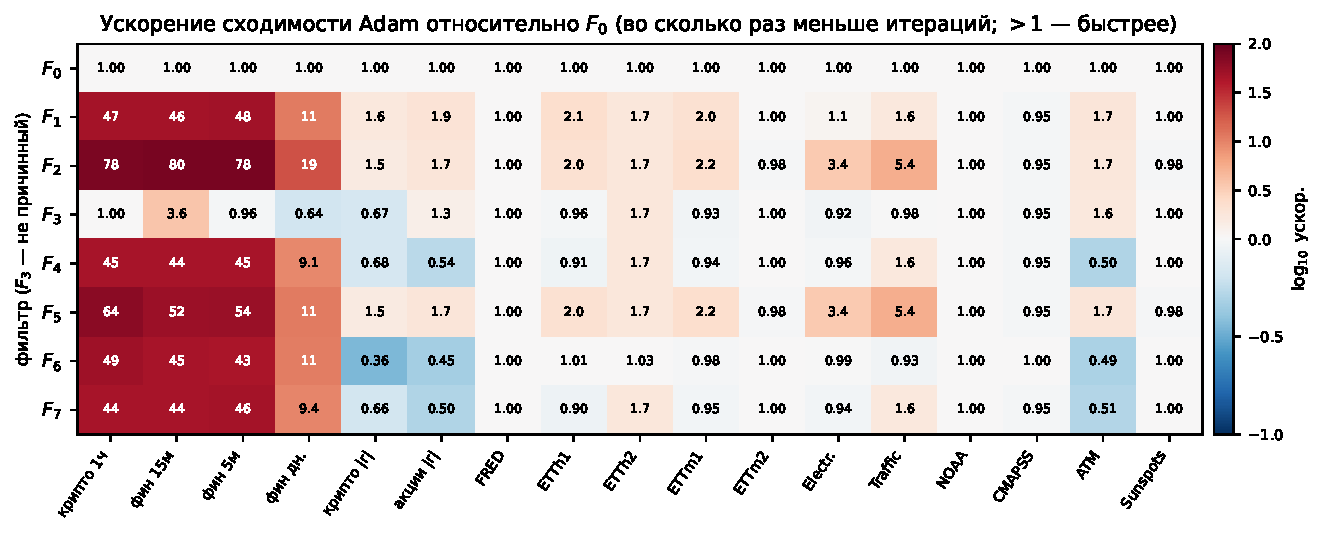
\includegraphics[width=\linewidth]{figures/new_datasets_heatmap.pdf}
\end{center}
Ускорение сходимости Adam относительно $F_0$ (Adam, регрессия AR(5)).
Выигрыш \textbf{сосредоточен на тяжёлохвостовых доходностях} (левый
блок): Калман $F_2$ ускоряет до $\mathbf{80\times}$, каскад $F_5$ ---
$\mathbf{64\times}$. На головном домене (крипто 1ч) $F_0$ сходится лишь
в $3/8$ прогонов, $F_2$ и $F_5$ --- во всех $8/8$. На
светлохвостовых/гладких рядах (FRED, ETT, NOAA, sunspots) все фильтры
$\approx1\times$ --- фильтровать не нужно.

% ----------------------- КОЛОНКА 4 -----------------------
\heading{Правило выбора $(\hat\alpha,\hat H)\to$ фильтр}
\begin{center}\small
\begin{tabular}{@{}lccc@{}}
\toprule
сектор $(\hat\alpha,\hat H)$ & фильтр & доменов & макс.\\
\midrule
$\hat\alpha{\approx}2,\ \hat H{\approx}0.5$ & $F_0$ & --- & $1\times$\\
$\hat\alpha{\approx}2,\ \hat H{>}0.6$       & $F_1$ & 1/2 & $1.9\times$\\
$\hat\alpha{<}1.9,\ \hat H{\approx}0.5$     & $F_2$ & 5/10 & $\mathbf{80\times}$\\
$\hat\alpha{<}1.9,\ \hat H{>}0.6$           & $F_5,F_6$ & 1/3 & $1.6\times$\\
\bottomrule
\end{tabular}
\end{center}
По двум диагностикам на обучающем отрезке выбирается стартовая связка;
финальный выбор --- причинной walk-forward валидацией.

\heading{Выводы}
\begin{itemize}\setlength{\itemsep}{0.3\baselineskip}
\item Нелинейная порядковая статистика (медиана) восстанавливает
\textbf{конечную} эффективную дисперсию шума --- чего линейные фильтры
дать не могут.
\item Каскад $F_5$ и адаптивный $F_6$ закрывают смешанный режим ``тяжёлый
хвост $\cap$ долгая память''.
\item Тяжёлый хвост сам по себе \emph{не} повод фильтровать: если узкое
место не в сходимости, лучший выбор --- $F_0$.
\item Правило по $(\hat\alpha,\hat H)$ предсказывает связку
(фильтр, оптимизатор) на широкой корзине реальных доменов.
\end{itemize}

\vfill
{\small Код и данные: \texttt{github.com/Poogee/momo\_proj}}

\end{multicols}
\end{document}
